\documentclass{standalone}

\usepackage{graphicx}

\usepackage{tikz}

\usetikzlibrary{positioning}
\usetikzlibrary{arrows.meta}

\begin{document}

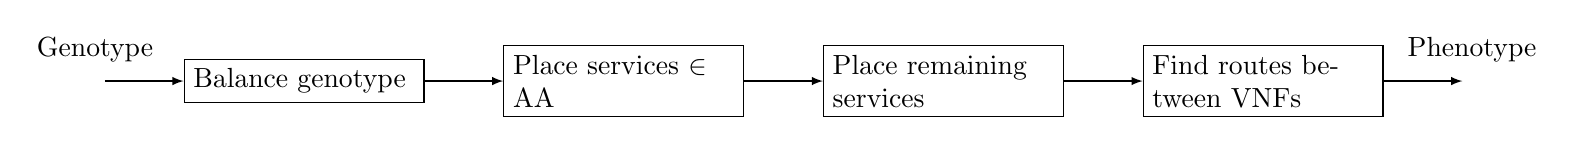
\begin{tikzpicture}[
    block/.style={rectangle, draw=black, fill=white, text width=8em},
]

    \node[] (H1) {};
    \node[] (T1) [above=0cm of H1] {Genotype};

    \node[block] (B1) [right=of H1] {Balance genotype};
    % \node[block] (B2) [right=of B1] {Swap services in AA to first VM of server};
    \node[block] (B3) [right=of B1] {Place services $\in$ AA};
    \node[block] (B4) [right=of B3] {Place remaining services};
    \node[block] (B5) [right=of B4] {Find routes between VNFs};

    \node[] (H2) [right=of B5] {};
    \node[] (T2) [above=0cm of H2] {Phenotype};

    \draw[-latex] (H1.east) -- (B1.west);
    \draw[-latex] (B1.east) -- (B3.west);
    % \draw[-latex] (B2.east) -- (B3.west);
    \draw[-latex] (B3.east) -- (B4.west);
    \draw[-latex] (B4.east) -- (B5.west);
    \draw[-latex] (B5.east) -- (H2.west);

\end{tikzpicture}

\end{document}